\documentclass{beamer}
\usefonttheme[onlymath]{serif}

\usepackage[utf8]{inputenc}
\usepackage[english]{babel}
\usepackage{amsmath}
\usepackage{xcolor}
\usepackage{amsthm}
\usepackage{amsfonts}
\usepackage{amssymb}
\usepackage{mathtools}
\usepackage{tikz}
\usepackage{graphicx}
\usetikzlibrary{arrows, automata, graphs, shapes, decorations.pathreplacing, decorations.pathmorphing}

\newenvironment{ppl}{\fontfamily{pzc}\selectfont}{\par}

% define environments
\makeatletter
\newcommand*{\shifttext}[2]{
	\settowidth{\@tempdima}{#2}
	\makebox[\@tempdima]{\hspace*{#1}#2}
}
\makeatother
%\renewcommand{\labelenumi}{(\roman{enumi})}
\newcommand{\equalhat}{\mathrel{\widehat{=}}}
\DeclareMathOperator{\spn}{span}
\newcommand{\ssqcup}{\mathrel{\shifttext{2pt}{$\sqcup$}\shifttext{-1.5pt}{$\sqcup$}}}

\newtheorem{thm}{Theorem}
\newtheorem{lem}{Lemma}

\definecolor{proof}{HTML}{75008C}
\definecolor{def}{HTML}{0000FF}
\definecolor{remark}{HTML}{389A39}
\definecolor{highlight}{HTML}{CE9E00}
\definecolor{grey}{HTML}{666666}
\newcommand{\defi}[1]{{\color{def}#1}}

% theme
\usetheme{Boadilla}
\useinnertheme{circles}
\setbeamertemplate{blocks}[rounded][shadow=false]
\setbeamercolor{block title}{fg=white, bg=blue!70}
\setbeamercolor{block body}{fg=black, bg=blue!15}
\beamertemplatenavigationsymbolsempty

% title page
\title[Übung 10]{FoSAP - Übung 10}
%\subtitle[Seminar on Mathematical Optimization]{Seminar on Mathematical Optimization in Summer Term 2017}
%\author[Niklas Rieken]{Niklas Rieken}
%\institute[RWTH Aachen]{RWTH Aachen}
%\date{June 13, 2017}
%\logo{\pgfimage[width=2cm,height=2cm]{}}
%\titlegraphic{\includegraphics[width=2cm,height=2cm]{}}
%\subject{}
%\keywords{}

% and here we go
\begin{document}

\begin{frame}{Aufgabe I1}
	\begin{itemize}
		\item[a)] Die Sprache $L_1 = \{a^i b^j \mid i+j \leq 200, 2i+j \geq 15\}$ ist nicht regulär.\pause
		\item[] \begin{ppl}$L_1$ nicht regulär: Sei $15 \leq n \leq 100$. Sei $w = a^n b^n$. $w \in L$. Wir betrachten eine Zerlegung $w = xyz$ mit $\left|xy\right| \leq n$ und $\left|y\right| > 0$. Wegen Pumping-Lemma muss auch $xy^iz \in L$ für alle $i$. Das Wort $xy^{200}z$ hat Länge ungefähr 200 und somit zu viele $a$ und $b$. So gilt $xy^{200}z \notin L$. Also $L$ nicht regulär und Aussage wahr.\end{ppl}\pause
		\alert<+->{$n$ fest gewählt, für $n > 200$ gibt es kein passendes Wort zum widerlegen mehr, da $L_1$ endlich ist. Jede endliche Sprache ist regulär.}
	\end{itemize}
\end{frame}


\begin{frame}{Aufgabe I1}
	\begin{itemize}
		\item[b)] Die Sprache $L_2 = \{(abcd)^n \mid n \in \mathbb{N}\}$ ist regulär.\pause
		\item[] \begin{ppl}Sei $n$ belibig. Wir wählen $w = (abcd)^n$. Es gilt $w \in L$. $x = ab, y = cd, z = (abcd)^{n-1}$. Es gilt $w=xyz$ und $\left| xy \right| \leq n$ und $|y| > 0$. Nach dem Pumping-Lemma muss auch $xy^iz \in L$. Es gilt $xy^2z = abcdcd(abcd)^{n-1} \notin L$. So mit $L_2$ nicht regulär und wiederlegt.\end{ppl}\pause
		\alert<+->{Zerlegung wurde fest gewählt. Die gewünschte Aussage gilt nicht für alle Zerlegungen ($x = \varepsilon, y = abcd, z = (abcd)^{n-1}$ kann man pumpen ohne die Sprache zu verlassen). Die Sprache $L_2$ ist regulär, da sie durch den regulären Ausdruck $(abcd)^\ast$ beschrieben wird.}
	\end{itemize}
\end{frame}


\begin{frame}{Aufgabe I1}
	\begin{itemize}
		\item[c)] Die Sprache $L_3 = \{z = xyx^R \mid x, y \in \Sigma^\ast\}$ mit $\Sigma = \{a, b, c\}$ ist kontextfrei.\pause
		\item[ ]\begin{ppl}$z=a^nb^na^n$, dann gibt's Zerlegung $z = uvwxy$ mit $|vwx| \leq n$ und $|vx| > 0$. Sei $uvwxy$ so gewählt, dass der $vxw$-Part im ersten drittel liegt, also nur die ersten $a$s enthält. Nach dem Pump-Lemma muss auch $uv^iwx^iy \in L$ für alle $i$ kann aber trivialistischerweise nicht sein da die Anzahl der $a$ am Anfang sich ändert und am Ende des Wortes gleich bleibt. $\implies L_3$  nicht konteckstfrei und die Ausage widerlegt.\end{ppl}\pause
		\alert<+->{Wieder Zerlegung fest gewählt. Außerdem wurde angenommen, dass $a^m b^n a^n \notin L_3$ für $m \neq n$, tatsächlich ist jedoch $L_3 = \Sigma^\ast$ und somit regulär.}
	\end{itemize}
\end{frame}

\begin{frame}{Synchronisierte und Unsynchronisierte Produkte} 
	\begin{itemize}
		\item[] Bekannt: Einfache Produktkonstruktion zum Erkennen von Schnitt, Vereinigung, etc. regulärer Sprachen
		\begin{figure}
			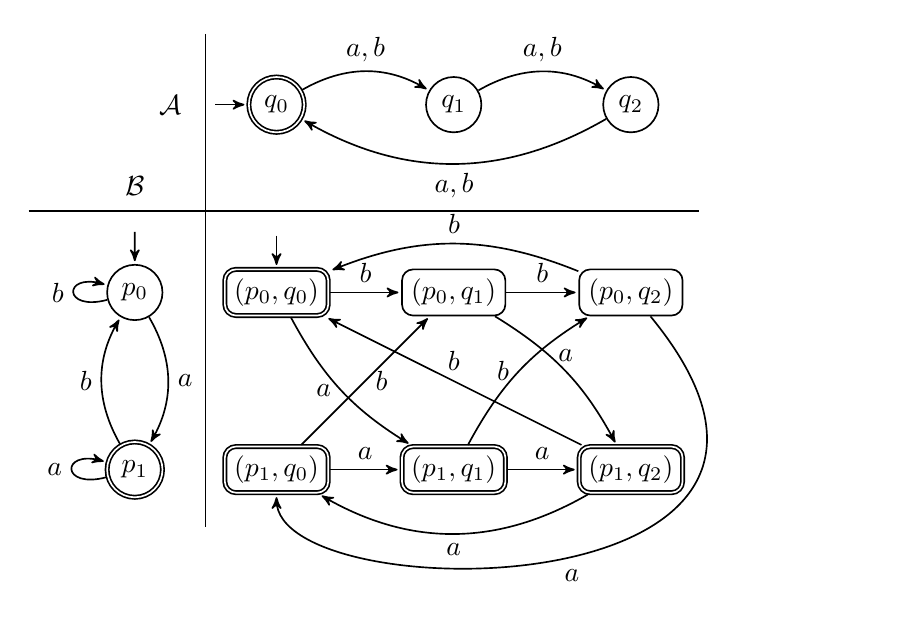
\begin{tikzpicture}[->, >=stealth', shorten >=1pt, auto, node distance=2.8cm, semithick, every state/.style={inner sep=0pt, minimum size=20pt}, scale=.9]
				\node[initial, initial text=, state, accepting]	(q0)	at (0, 0)		{$q_0$};
				\node[state]										(q1) at (2.5, 0)		{$q_1$};
				\node[state]										(q2) at (5, 0)		{$q_2$};
				\node (A) at (-1.5, 0) {$\mathcal{A}$};
	
				\path	(q0) edge[bend left] node {$a, b$} (q1)
						(q1) edge[bend left] node {$a, b$} (q2)
						(q2) edge[bend left] node {$a, b$} (q0);
	
				\begin{scope}[yshift=-0.15cm]
					\node[initial above, initial text=, state]		(p0)	 at (-2, -2.5)	{$p_0$};
					\node[state, accepting]							(p1) at (-2, -5)		{$p_1$};
					\node (B) at (-2, -1) {$\mathcal{B}$};
	
					\path	(p0) edge[bend left] node {$a$} (p1)
							(p0) edge[loop left] node {$b$} (p0)
							(p1) edge[loop left] node {$a$} (p1)
							(p1) edge[bend left] node {$b$} (p0);
				\end{scope}
		
				\draw[-] (-1, 1) -- (-1, -6);
				\draw[-] (-3.5, -1.5) -- (6, -1.5);

\uncover<2->{	\begin{scope}[state/.style={draw, rectangle, rounded corners}, yshift=-0.15cm]
					\node[initial above, initial text=, state, accepting]	(p0q0)	at (0, -2.5)		{$(p_0, q_0)$};
					\node[state]												(p0q1)	at (2.5, -2.5)		{$(p_0, q_1)$};
					\node[state]												(p0q2)	at (5, -2.5)		{$(p_0, q_2)$};
					\node[state, accepting]									(p1q0)	at (0, -5)		{$(p_1, q_0)$};
					\node[state, accepting]									(p1q1)	at (2.5, -5)		{$(p_1, q_1)$};
					\node[state, accepting]									(p1q2)	at (5, -5)		{$(p_1, q_2)$};
		
					\path	(p0q0) edge[bend right=15] node[left] {$a$} (p1q1)
							(p0q0) edge node {$b$} (p0q1)
							(p0q1) edge[bend left=15] node[above] {$a$} (p1q2)
							(p0q1) edge node {$b$} (p0q2)
							%(p0q2) edge node {$a$} (p1q0)
							(p0q2) edge[bend right=22] node[above] {$b$} (p0q0)
							(p1q0) edge node {$a$} (p1q1)
							(p1q0) edge node[right] {$b$} (p0q1)
							(p1q1) edge node {$a$} (p1q2)
							(p1q1) edge[bend left=15] node[left] {$b$} (p0q2)
							(p1q2) edge[bend left] node {$a$} (p1q0)
							(p1q2) edge node[above] {$b$} (p0q0);
				
					\draw (p0q2) .. controls (8.7, -7) and (0, -7) .. node {$a$} (p1q0);
				\end{scope}	
}
			\end{tikzpicture}
		\end{figure}
	\end{itemize}
\end{frame}


\begin{frame}{Synchronisierte und Unsynchronisierte Produkte} 
	\begin{itemize}
		\item[] Jetzt: Synchronisiertes Produkt: $\mathcal{A} \circ \mathcal{B}$ mit $\Sigma_\circ = \{a\}$.
		\begin{figure}
			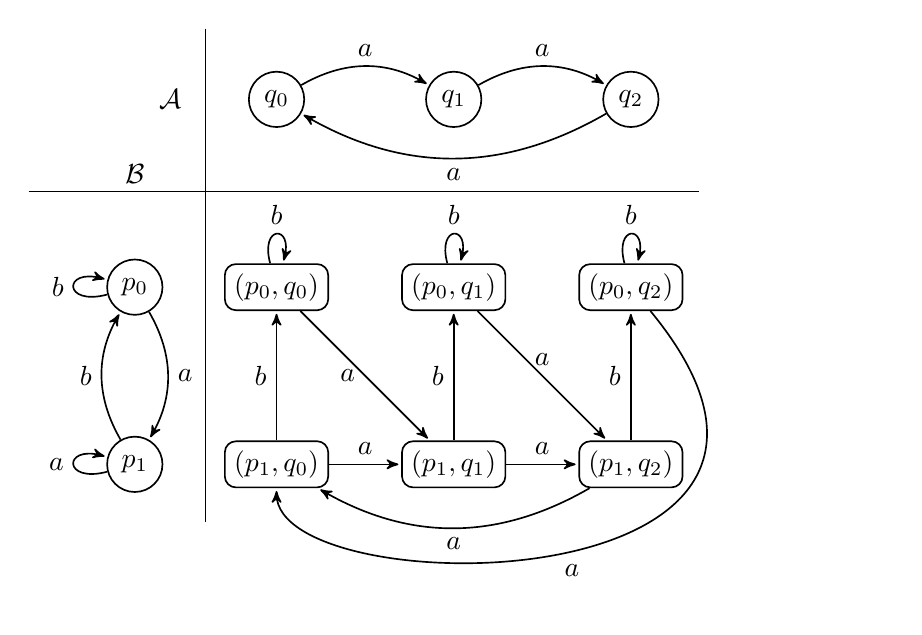
\begin{tikzpicture}[->, >=stealth', shorten >=1pt, auto, node distance=2.8cm, semithick, every state/.style={inner sep=0pt, minimum size=20pt}, scale=.9]
				\node[state]		(q0) at (0, 0)		{$q_0$};
				\node[state]		(q1) at (2.5, 0)		{$q_1$};
				\node[state]		(q2) at (5, 0)		{$q_2$};
				\node (A) at (-1.5, 0) {$\mathcal{A}$};
	
				\path	(q0) edge[bend left] node {$a$} (q1)
						(q1) edge[bend left] node {$a$} (q2)
						(q2) edge[bend left] node {$a$} (q0);
	
				\begin{scope}[yshift=-0.15cm]
					\node[state]		(p0)	 at (-2, -2.5)	{$p_0$};
					\node[state]		(p1) at (-2, -5)		{$p_1$};
					\node (B) at (-2, -.9) {$\mathcal{B}$};
	
					\path	(p0) edge[bend left] node {$a$} (p1)
							(p0) edge[loop left] node {$b$} (p0)
							(p1) edge[loop left] node {$a$} (p1)
							(p1) edge[bend left] node {$b$} (p0);
				\end{scope}
		
				\draw[-] (-1, 1) -- (-1, -6);
				\draw[-] (-3.5, -1.3) -- (6, -1.3);

\uncover<2->{	\begin{scope}[state/.style={draw, rectangle, rounded corners}, yshift=-0.15cm]
					\node[state]		(p0q0)	at (0, -2.5)		{$(p_0, q_0)$};
					\node[state]		(p0q1)	at (2.5, -2.5)	{$(p_0, q_1)$};
					\node[state]		(p0q2)	at (5, -2.5)		{$(p_0, q_2)$};
					\node[state]		(p1q0)	at (0, -5)		{$(p_1, q_0)$};
					\node[state]		(p1q1)	at (2.5, -5)		{$(p_1, q_1)$};
					\node[state]		(p1q2)	at (5, -5)		{$(p_1, q_2)$};
		
					\path	(p0q0) edge node[left] {$a$} (p1q1)
							(p0q0) edge[loop above] node {$b$} (p0q0)
							(p0q1) edge node[above] {$a$} (p1q2)
							(p0q1) edge[loop above] node {$b$} (p0q1)
							%(p0q2) edge node {$a$} (p1q0)
							(p0q2) edge[loop above] node {$b$} (p0q2)
							(p1q0) edge node {$a$} (p1q1)
							(p1q0) edge node {$b$} (p0q0)
							(p1q1) edge node {$a$} (p1q2)
							(p1q1) edge node {$b$} (p0q1)
							(p1q2) edge[bend left] node {$a$} (p1q0)
							(p1q2) edge node {$b$} (p0q2);
				
					\draw (p0q2) .. controls (8.7, -7) and (0, -7) .. node {$a$} (p1q0);
				\end{scope}	
}
			\end{tikzpicture}
		\end{figure}
	\end{itemize}
\end{frame}

\begin{frame}{Synchronisierte und Unsynchronisierte Produkte} 
	\begin{itemize}
		\item[] Unsynchronisiertes Produkt: $\mathcal{A} \ssqcup \mathcal{B}$.
		\begin{figure}
			\begin{tikzpicture}[->, >=stealth', shorten >=1pt, auto, node distance=2.8cm, semithick, every state/.style={inner sep=0pt, minimum size=20pt}, scale=.9]
				\node[state]		(q0) at (0, 0)		{$q_0$};
				\node[state]		(q1) at (2.5, 0)		{$q_1$};
				\node[state]		(q2) at (5, 0)		{$q_2$};
				\node (A) at (-1.5, 0) {$\mathcal{A}$};
	
				\path	(q0) edge[bend left] node {$a$} (q1)
						(q1) edge[bend left] node {$a$} (q2)
						(q2) edge[bend left] node {$a$} (q0);
	
				\begin{scope}[yshift=-0.15cm]
					\node[state]		(p0)	 at (-2, -2.5)	{$p_0$};
					\node[state]		(p1) at (-2, -5)		{$p_1$};
					\node (B) at (-2, -.9) {$\mathcal{B}$};
	
					\path	(p0) edge[bend left] node {$a$} (p1)
							(p0) edge[loop left] node {$b$} (p0)
							(p1) edge[loop left] node {$a$} (p1)
							(p1) edge[bend left] node {$b$} (p0);
				\end{scope}
		
				\draw[-] (-1, 1) -- (-1, -6);
				\draw[-] (-3.5, -1.3) -- (6, -1.3);

\uncover<2->{	\begin{scope}[state/.style={draw, rectangle, rounded corners}, yshift=-0.15cm]
					\node[state]		(p0q0)	at (0, -2.5)		{$(p_0, q_0)$};
					\node[state]		(p0q1)	at (2.5, -2.5)	{$(p_0, q_1)$};
					\node[state]		(p0q2)	at (5, -2.5)		{$(p_0, q_2)$};
					\node[state]		(p1q0)	at (0, -5)		{$(p_1, q_0)$};
					\node[state]		(p1q1)	at (2.5, -5)		{$(p_1, q_1)$};
					\node[state]		(p1q2)	at (5, -5)		{$(p_1, q_2)$};
		
					\path	(p0q0) edge[loop above] node {$b$} (p0q0)
							(p0q1) edge[loop above] node {$b$} (p0q1)
							(p0q2) edge[loop above] node {$b$} (p0q2)
							(p1q0) edge[bend left] node {$b$} (p0q0)
							(p1q1) edge[bend left] node {$b$} (p0q1)
							(p1q2) edge[bend left] node {$b$} (p0q2);
}						
\uncover<3->	{		\path[red]	(p0q0) edge[bend left] node {$a$} (p1q0)
							(p0q1) edge[bend left] node {$a$} (p1q1)
							(p0q2) edge[bend left] node {$a$} (p1q2)
							(p1q0) edge[loop below] node {$a$} (p1q0)
							(p1q1) edge[loop below] node {$a$} (p1q1)
							(p1q2) edge[loop below] node {$a$} (p1q2);
}
\uncover<3->	{		\path[blue]	(p1q0) edge node {$a$} (p1q1)
							(p1q1) edge node {$a$} (p1q2)
							(p1q2) edge[bend left=45] node[below] {$a$} (p1q0)
							(p0q0) edge node {$a$} (p0q1)
							(p0q1) edge node {$a$} (p0q2)
							(p0q2) edge[bend right] node[above, near end] {$a$} (p0q0);
}
\uncover<2->{		
				\end{scope}	
}
			\end{tikzpicture}
		\end{figure}
	\end{itemize}
\end{frame}


\begin{frame}{Kontextsensitive Grammatiken}
	\begin{itemize}
		\item Bisher: Kontextfreie Grammatiken: $\mathcal{G} = (N, \Sigma, P, S)$ mit Produktionen der Form $A \to \gamma$ mit $\gamma \in (N \cup \Sigma)^\ast$.\pause
		\item Jetzt: Mit Kontextsensitive Grammatiken, d.h. erlaube die Anwendung von Produktionen nur mit bestimmten Kontext:
			$$
				\alpha A \beta \to \alpha \gamma \beta, \quad\quad\quad \alpha, \beta \in (N \cup \Sigma)^\ast, \gamma \in (N \cup \Sigma)^+.
			$$\pause
		\item Kontextsensitive Grammatik für $\{a^n b^n c^n \mid n \in \mathbb{N}\}$:
			\begin{align*}
				S &\to aSBC \mid \varepsilon, & CB &\to XB, & XB &\to XY,\\
				XY &\to BY, & BY &\to BC, & aB &\to ab,\\
				bB &\to bb, &  C &\to c.
			\end{align*}\pause
		\item Wie könnte ein Automatenmodell, das kontextsensitive Sprachen erkennt, funktionieren?
	\end{itemize}
\end{frame}

% eof
\end{document}